\section{OpenFOAM}\label{sec:3_openfoam}
%
Las flujometrías se realizaron con \emph{OpenFOAM}, un software de
Fluidodinámica Computacional, o CFD por sus siglas en inglés, de código libre y
abierto escrito en ``C++''.
%
% La herramienta seleccionada para realizar las flujometrías es OpenFOAM, por ser
% una herramienta libre y de código abierto.
%
Junto con este programa se utilizaron otras herramientas libres para generar la
geometría a modelar y post-procesar los resultados..
%
El esquema de trabajo para realizar las simulaciones consistió en:

\begin{enumerate}
        %
    \item Pre-procesado
      %

        \begin{enumerate}
                %
            \item Definir la geometría a analizar.
              %
            \item Generar una malla con un tamaño de elemento adecuado (la
solución a problemas de CFD depende fuertemente de la cantidad y tamaño de
celdas utilizadas).
              %
            \item Seleccionar los modelos adecuados.
              %
            \item Definir las propiedades del fluido.
              %
            \item Definir las condiciones de borde.

              %
        \end{enumerate}
        %
    \item Solver
      %
    \begin{enumerate} \item Seleccionar el solver a utilizar.
            %
            \item Ejecutar la simulación.
            %
    \end{enumerate}
        %
\item Post-procesado
      %
    \begin{enumerate}
                %
        \item Visualizar los resultados de las distintas variables de la
            simulación.
            %
        \item Extraer la información necesaria.
            %
    \end{enumerate}
        %
\end{enumerate}

%%%%%%%%%%%%%%%%%%%%%%%%%%%%%%%%%%%%%%%%%%%%%%%%%%%%%%%%%%%%%%%%%%%%%%%%%%%%%%%

\subsection{Pre-procesado}
%
El preprocesado consiste en definir geometría y condiciones iniciales de la
simulación a partir de los datos obtenidos de las simulaciones con el
optimizador e ICESym.
%
Con los resultados del simulador se grafica la diferencia de presión entre el
puerto de admisión o escape y la cámara correspondiente en función de la apertura
del puerto, para un rango de velocidades de 1000 a 9000 RPM, con el fin de
identificar las zonas en las condiciones operativas en las que evaluar el puerto.
%
En la Figura~\ref{fig:puntos_interes} se muestra una gráfica de $\Delta P$ y
alzada para los puertos de admisión y escape del motor resultante de la primera
iteración (con un $C_{D}$ constante).

Como es de esperarse se tienen mayores diferenciales de presión a menores
aperturas del puerto porque se está próximo a los eventos de apertura o cierre
del mismo.
%
A diferencia del puerto de admisión, en el puerto de escape se ve una banda
bastante definida de operación que se hace más ``llena'' a medida que aumenta el
área del puerto expuesta a la cámara (alzada).
%
Durante la apertura del puerto se ven las mayores diferencias de presión en las
que hay dos bandas bien definidas.
%
Se toman algunos puntos arriba en la zona con mayor $\Delta P$ y una cantidad
menor para velocidades con $\Delta P \simeq 0$.
%
A medida que el puerto se abre la diferencia de presión con el gas en la cámara
disminuye y esta banda se afina.

% \begin{figure}
%     \centering
%     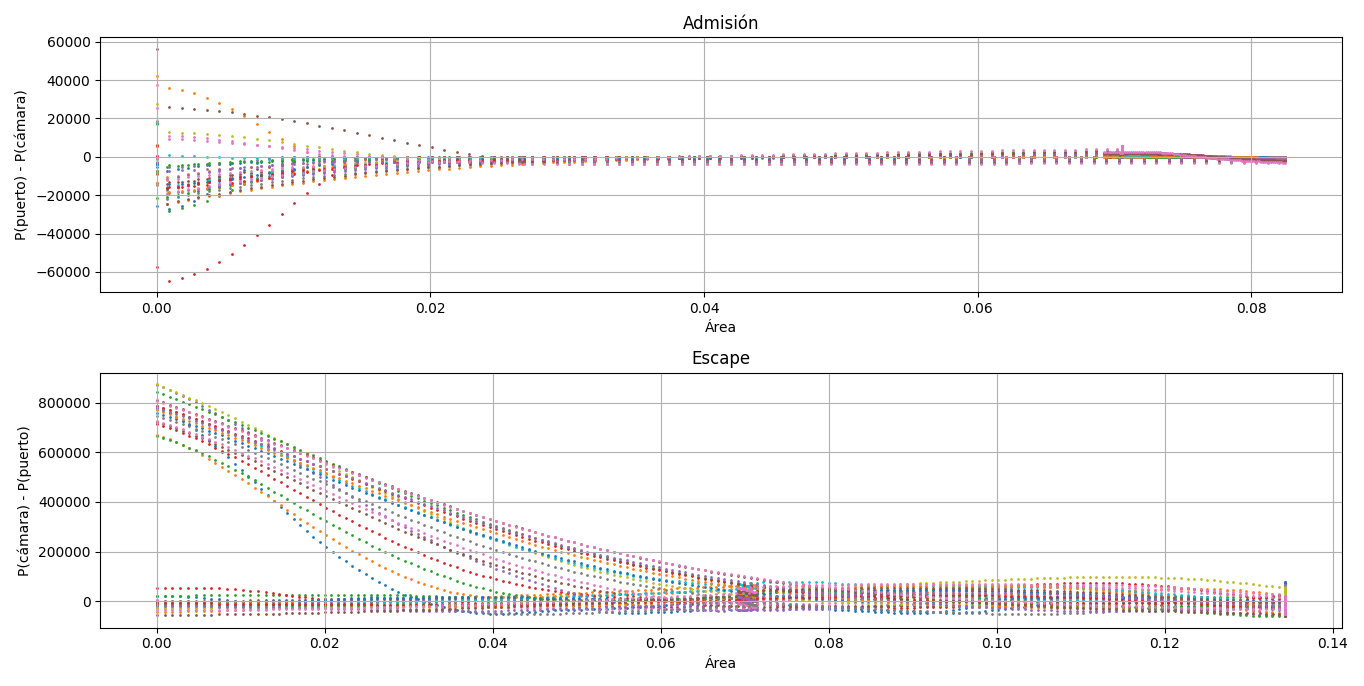
\includegraphics[width=\textwidth]{flujometrias/puntos_de_interes.png}
%     \caption{Presión en función de la apertura el puerto,
% $\Delta P = f(l_{v})$}\label{fig:puntos_interes}
% \end{figure}

El valor de alzada está directamente relacionado con la posición angular del
cigüeñal, por lo que una vez seleccionados los puntos de interés se puede
extraer la geometría deseada de un modelo de CAD paramétrico del motor.
%
En este modelo se representó la mitad de la geometría que contiene los puertos
de admisión y escape, y se obtuvo realizando operaciones geométricas con los
volúmenes que representan diferentes componentes del motor como son el estator,
rotor, paletas, etc.
%
% En la Figura~\ref{fig:admision_50} se muestra parte del proceso para obtener el
% puerto de admisión a $\theta=50^{\circ}$, en donde se suma el volumen del mismo
% en gris y las Figuras que se restan que corresponden al rotor, las paletas y un
% paralelogramo para quitar una región que no se simuló.

\begin{figure}
    \centering
    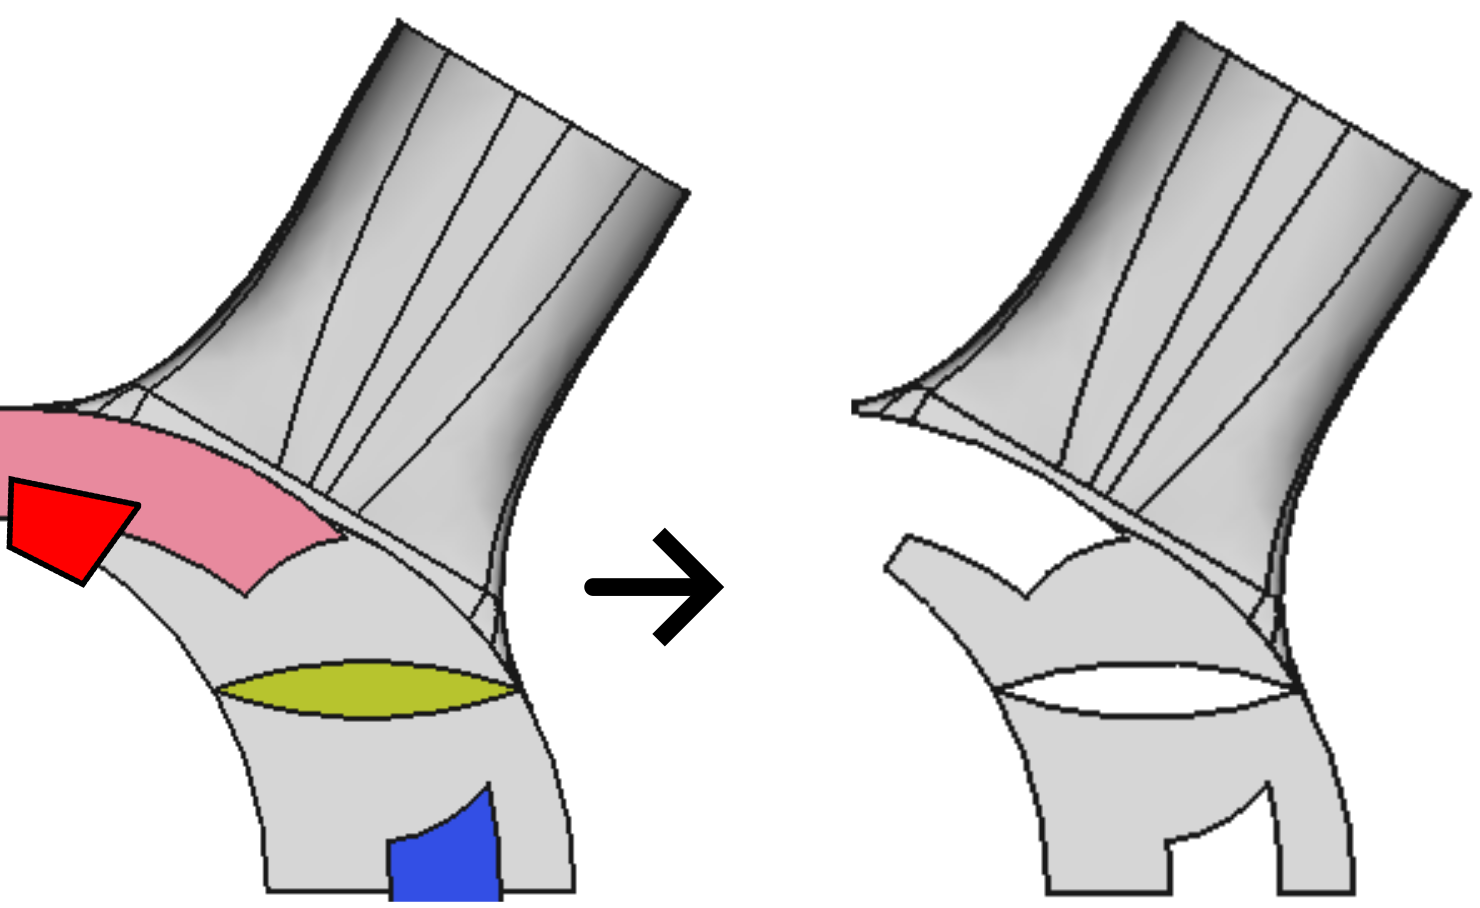
\includegraphics[width=0.7\textwidth]{./CAD/freecad_pasos.png}
    \caption{Puerto de admisión para $\theta=50^{\circ}$ modelado con
FreeCAD}\label{fig:admision_50}
\end{figure}

Esta geometría fue generada por el programa FreeCAD~\parencite{freecad},
exportada a un archivo
``.BREP''\footnote{\href{https://dev.opencascade.org/doc/overview/html/specification\_\_brep\_format.html}{Formato
BREP, opencascade.org}} para luego ser importada en Salome\parencite{salome},
que se utiliza para generar una malla cerrada, hermética, que puede ser
procesada por los complementos de OpenFOAM utilizados para generar la malla de
la simulación.
%
Es importante que se satisfaga la hermeticidad de la malla, lo cual significa
que los nodos en la frontera entre superficies coincidan, como se puede observar
en la Figura~\ref{fig:salome_malla_hermetica}, en la que se ven dos superficies
``walls'' y ``outlet'' y los nodos compartidos entre ambas superficies.
%

\begin{figure}[ht]
    \centering
    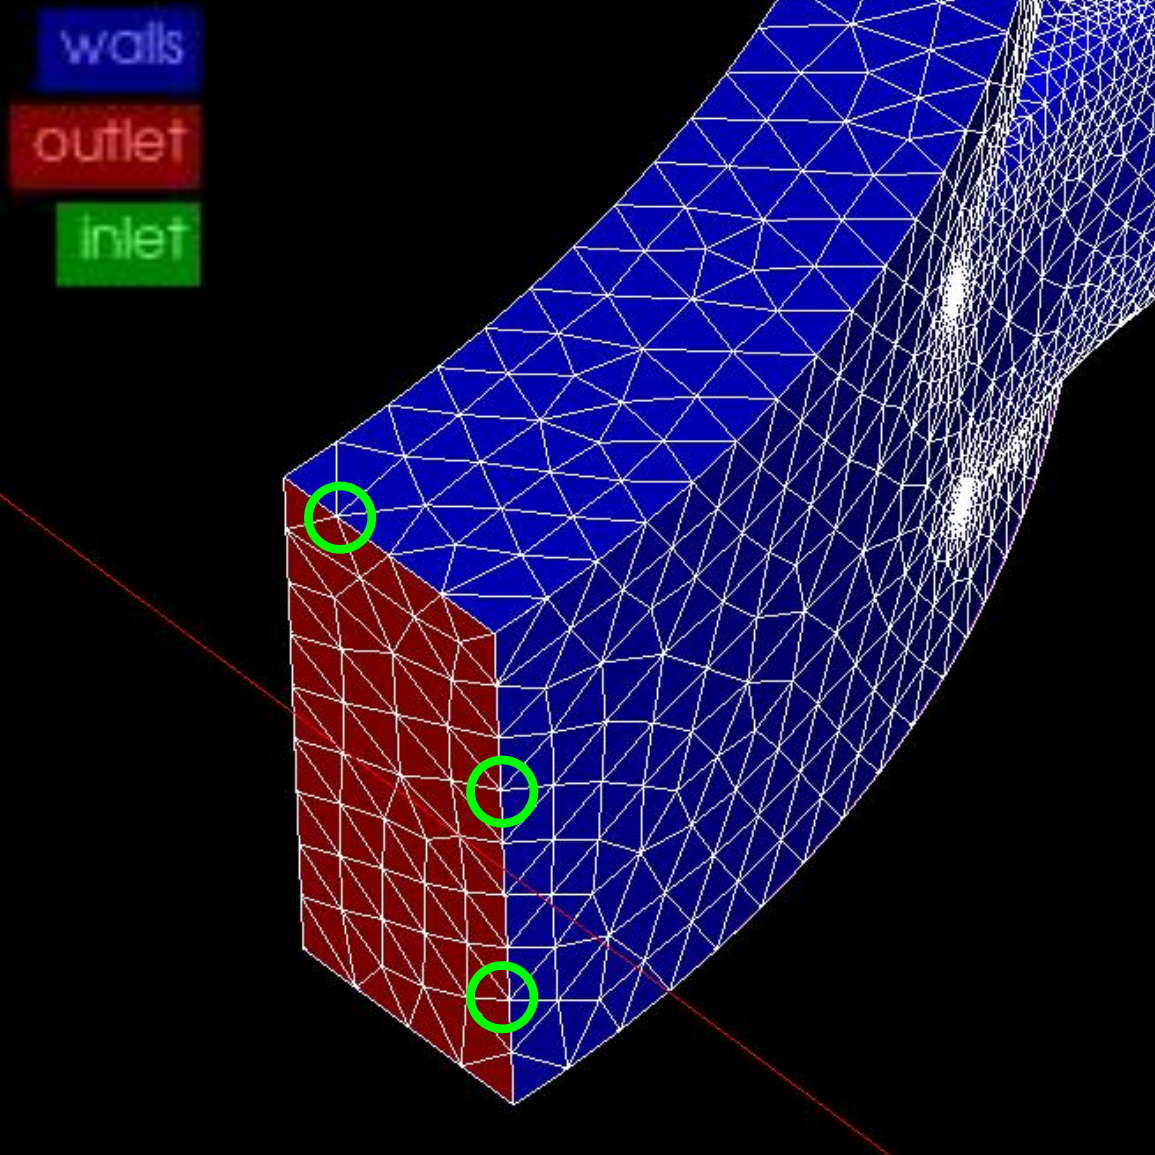
\includegraphics[width=0.5\textwidth]{./flujometrias/salome_malla_hermetica.png}
    \caption{Malla hermética}\label{fig:salome_malla_hermetica}
\end{figure}

El proceso en Salome consta de importar la geometría generada por FreeCAD y
separar la misma en superficies utilizadas para definir condiciones de contorno
en OpenFOAM.
%
Las superficies diferenciadas son: puerto, cámara/s y pared, ver
Figura~\ref{fig:openfoam_parches}.

\begin{figure}[ht]
    \centering
    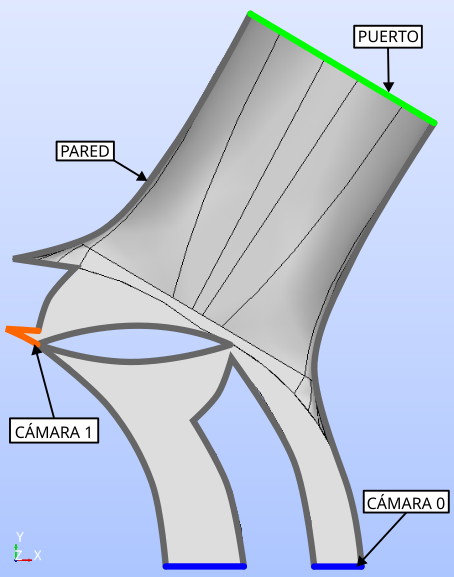
\includegraphics[width=0.7\textwidth]{./flujometrias/openfoam_parches.png}
    \caption{Nombres de Parches}\label{fig:openfoam_parches}
\end{figure}

Luego de separadas estas superficies se procede a generar la malla en formato
ASCII STL con el complemento de mallado de Salome.
%
Se utilizó el generador de mallas NETGEN 1D-2D para crear la superficie, en
general se configuró el software de modo de tener un stl de buena calidad con
elementos de menor tamaño en zonas de mayor curvatura.
%
En la Figura~\ref{fig:salome_fina_gruesa} se ve la diferencia en cantidad de
nodos de dos mallas, una malla fina a la izquierda y una malla gruesa a la
derecha.
%
En la Tabla~\ref{tab:salome_fina_gruesa} se muestra la diferencia entre algunos
parámetros básicos de configuración para las dos mallas.
%
% Esto sin requerir de una gran cantidad de elementos para no ralentizar el
% procesado con SnappyHexMesh.

\begin{figure}[t!]
    \centering
    \begin{subfigure}[t]{0.5\textwidth}
        \centering
        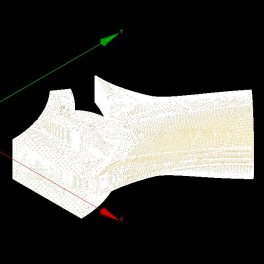
\includegraphics{/flujometrias/salome3_fina.png}
        \caption{Malla fina sin optimizar}
    \end{subfigure}%
    \begin{subfigure}[t]{0.5\textwidth}
        \centering
        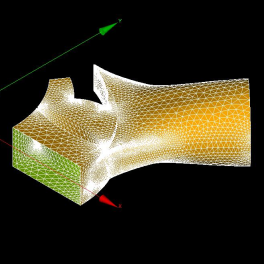
\includegraphics{/flujometrias/salome3_gruesa.png}
        \caption{Malla gruesa optimizada}
    \end{subfigure}
    \caption{Diferentes mallas para flujometrías}\label{fig:salome_fina_gruesa}
\end{figure}

\begin{table}
    \centering
    \begin{tabular}{lccc} \toprule
        Parámetro                & Malla Fina    & Malla Gruesa     & Unidades\\ \midrule
        Tamaño máximo            & 0,001         & 0,03             & m \\
        Tamaño mínimo            & 1E-7          & 2,4E-5           & m \\
        Limitado por curvatura   & Sí            & Sí               & - \\
        Optimizar                & No            & Sí               & - \\
        Cantidad de nodos        & 99311         & 49112            & - \\
        Cantidad de elementos    & 204695        & 103163           & - \\ \bottomrule
    \end{tabular}
    \caption{Configuración de mallas mostradas en la Figura~\ref{fig:salome_fina_gruesa}}
    \label{tab:salome_fina_gruesa}
\end{table}


\subsubsection{Configuración}
%
Para conFigurar una simulación de OpenFOAM se organiza el directorio de
simulación como se indica en la Figura~\ref{fig:direc_pf} para las flujometrías
de aire considerado como incompresible  y~\ref{fig:direc_rpf} en los casos en
los que se tiene en cuenta la compresibilidad del aire.
%
Cada directorio contiene una carpeta con condiciones iniciales ``0'', malla
``constant'', conFiguraciones particulares de cada solver ``system'' y una
caperta con los resultados del post-procesado el cual se puede realizar
durante cada paso de simulación o al final del proceso dependiendo de la
configuración que se haya utilizado.

\begin{figure}[ht!]
  \centering
  \begin{subfigure}[b]{0.4\textwidth}
    \centering
    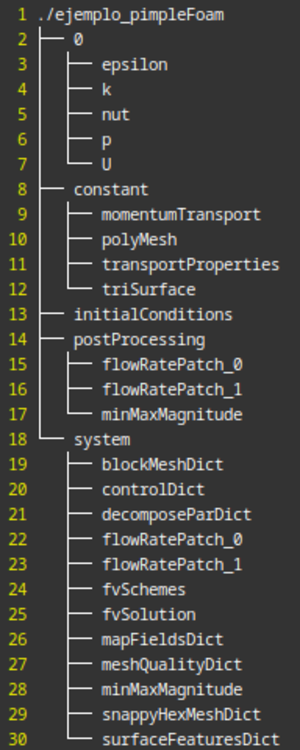
\includegraphics{flujometrias/direct_pimplefoam.pdf}
    \caption{\emph{pimpleFoam}\label{fig:direc_pf} }
  \end{subfigure}%
  \begin{subfigure}[b]{0.4\textwidth}
    \centering
    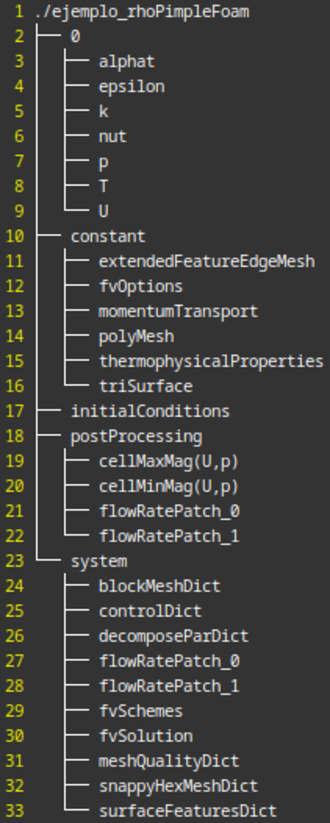
\includegraphics{flujometrias/direct_rhopimplefoam.pdf}
    \caption{\emph{rhoPimpleFoam}\label{fig:direc_rpf} }
  \end{subfigure}
  \caption{Esquema de directorios OpenFOAM}
\end{figure}


En el directorio ``0'' se indican las condiciones iniciales y de borde de cada
simulación, utilizando una configuración genérica con parámetros definidos en un
archivo separado.
%
Esto se realiza de este modo para aprovechar las características paramétricas de
OpenFOAM, permitiendo ejecutar una gran cantidad de simulaciones en serie
variando solamente los parámetros definidos en un archivo externo
``inital\_conditions.cc''.

Estos archivos de condiciones inciales se generan con un \emph{script} que toma
valores de las simulaciones de \emph{ICESym}, como se indicó en la
sección~\ref{cap2:cond_iniciales}, en la que también se detallan las ecuaciones
e hipótesis utilizadas para obtener dichos valores.
%
La ejecución de las simulaciones también se automatiza con scripts de
\emph{bash} con los pasos para ejecutar las corridas con \emph{ICESym}.
%
Con los resultados de las simulaciones se procede a calcular/leer la magnitud
del caudal másico, necesario para el cálculo del coeficiente de descarga.


\subsubsection{Malla}\label{sec:cap3_of_malla}
%
Una vez obtenido el archivo STL se procede a la generación de la malla dentro de
OpenFOAM con \emph{blockMesh} y \emph{snappyHexMesh}.
%
Primero se crea crea una malla con \emph{blockMesh} que  debe contener la
totalidad del volumen del puerto a simular, como se puede en la
Figura~\ref{fig:paraview_blockMesh_stl}.
%
En este paso se define el tamaño de base de la malla y el nivel general de
refinamiento.
%
A partir de estos hexaedros se produce el refinamiento por \emph{castelación}
que consiste en dividir las celdas en hexaedros más pequeños y luego aplicar el
\emph{snapping} para adaptarse a la superficie del volumen que se está
modelando, ver Figura~\ref{fig:openfoam_shm_pasos}.
%

\begin{figure}
    \centering
    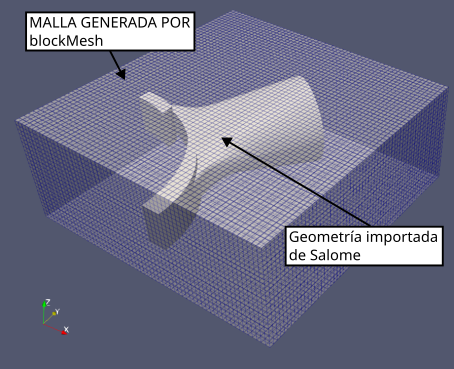
\includegraphics[width=0.5\textwidth]{flujometrias/paraview_blockMesh_stl.png}
    \caption{Malla de blockMesh y stl de Salome}\label{fig:paraview_blockMesh_stl}
\end{figure}

\begin{figure}[t!]
    \centering
    \begin{subfigure}[t]{0.5\textwidth}
        \centering
        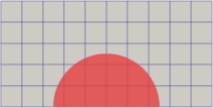
\includegraphics{flujometrias/shm_fondo.png}
        \caption{Malla de fondo y geometría}
    \end{subfigure}%
    \begin{subfigure}[t]{0.5\textwidth}
        \centering
        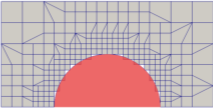
\includegraphics{flujometrias/shm_castelacion.png}
        \caption{Castelación}
    \end{subfigure}
    \begin{subfigure}[t]{0.5\textwidth}
        \centering
        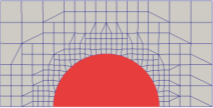
\includegraphics{flujometrias/shm_snapping.png}
        \caption{Snapping}
    \end{subfigure}
    \caption{Pasos de SnappyHexMesh\parencite{shm_steps}}\label{fig:openfoam_shm_pasos}
\end{figure}


El complemento \emph{blockMesh} crea una malla paramétrica con bloques, con
opciones para la creación de la malla con gradientes de tamaño de bloques y
diferentes opciones para los bordes, los cuales se pueden construir por líneas
rectas, arcos o ``splines''.
%
La malla se genera o conFigura con un diccionario \emph{blockMeshDict} ubicado
en \emph{constant/polyMesh}.

El complemento \emph{snappyHexMesh} es el segundo paso del mallado.
%
Parte de una malla de bloques como la generada con la utilidad \emph{blockMesh}
y la \emph{talla} para acomodarse a la geometría dada, generando una malla 3D
conformada por hexaedros y hexaedros partidos a partir de superficies de caras
triangulares en formato de \emph{estereolitografía} (STL por sus siglas en
inglés).
%
Además permite refinar zonas particulares de la geometría y crear un
refinamiento mayor en la zona de la capa límite.
